%% The following is a directive for TeXShop to indicate the main file
%%!TEX root = diss.tex

\chapter{Capacitively coupled quantum dot}
\label{ch:Methods}
\section{Quantum dots in GaAs/AlGaAs heterostructures}
\label{sec:qds}

The focus of this section will be the theory of double (and single) quantum dots in the 2 dimensional electron gas hosted by AlGaAs/GaAs. The basis of this section will be the Fig. \ref{fig:dqd}. In addition, there will be a discussion of the energy scales at play in the system and those that are most important for our entropy measurements.

\begin{figure}[h]
\centering
\resizebox{\textwidth}{!}{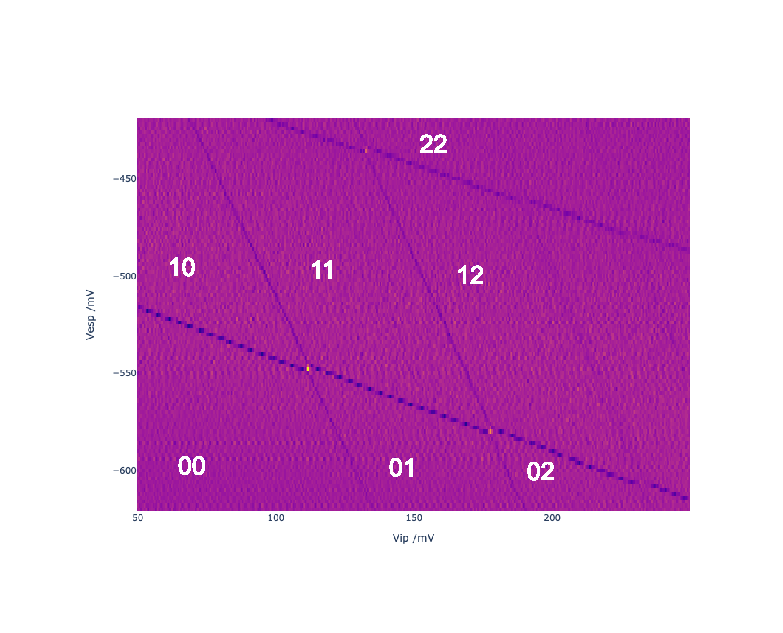
\includegraphics{figures/pdfs/dqd_temp.eps}}
\caption{The states of the double quantum dot system are mapped out by charge sensing the occupation of both dots. The color indicates the derivative of the current through the charge sensor. Sudden changes in this current indicate state changes in the two dots, with larger changes (seen as darker on this plot) indicating changes in the probe dot, and smaller changes (slightly lighter on this plot) indicating changes in states in the impurity dot. The large squares indicate regions of constant state in the two dots and are labelled by [occupation main dot, occupation impurity dot].}
\label{fig:dqd}       % Give a unique label to the figure. 
\end{figure}

\section{The device and measurement protocol}
\label{sec:device}
The measurement protocol as laid out in Fig.~\ref{fig:num_int} requires the ability to vary the temperature of the system. However, in practice, instability in the exact locations of $V_{mid}$ makes it difficult to accurately determine $\Delta S$ of the hot and cold curves independently. Because of this instability, it is necessary to oscillate between hot and cold as we measure over the transition. With this measurement scheme, any heating not localized on the device is not useful as it will take too long to equilibrate through the entirety of whatever larger system is being heated.

We are pursuing multiple possible solutions for fast localized heating. The first is the technique employed by Hartman et al. and used in previous device designs which involves directly injecting hot electrons into the electron reservoir coupled to the probe dot. This can be done by running a current through a QPC (tuned to be fairly resistive) pointed into the electron reservoir. When the current is turned off the heat in the electron reservoir is dissipated by coupling to phonons and connection to a `cold' ground - i.e. a much larger bath of electrons at lower temperature. By turning on and off the current running through this resistive heater QPC, we can locally control the temperature of the electrons in the system. Another possible technique that could be employed to allow for fast localized heating is heating the crystalline lattice of the substrate. With this technique, the electron-phonon coupling in the electron reservoir would ensure that the electrons quickly thermalize. Resistive heating would most likely be used to heat the phonons, either by electron phonon coupling using a QPC which is electrically insulated from the device, or by building a resistor on top of the substrate using a very long wire with some finite resistance.

Devices to complete this experiment will be built on GaAs/AlGaAs heterostructure which hosts a 2DEG (see Fig \ref{fig:algaas}). The 2DEG is electrostatically gated to allow for local control of the electron density i.e. by applying an electric field with an electrically isolated gate, the electron density of the 2DEG is controlled beneath this gate \cite{Kouwenhoven1997}. Ohmic contact is made with the 2DEG via a diffusive process of Ni/Au/Ge through the substrate. Gating structures will be defined using standard photolithography and electron beam lithography techniques.  

The next part of this section will focus on breaking down the various gates in use on the device and their roles. Relevant length scales, etc. will be discussed. This section is focussed around Fig. \ref{fig:device}. Connections will be made to the previous section, pointing out the energy scales in our system and how they were calculated.

\begin{figure}[h]
\centering
\resizebox{\textwidth}{!}{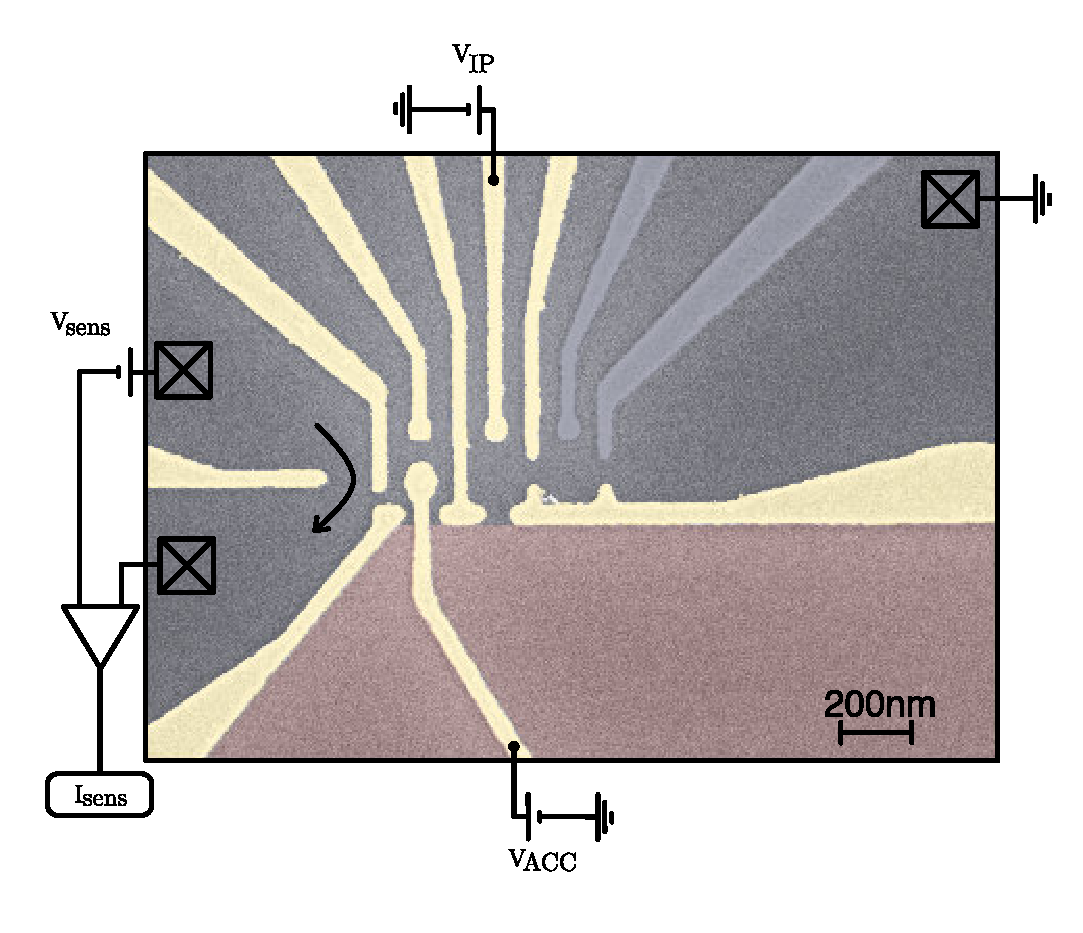
\includegraphics{figures/pdfs/small_dots_2.eps}}
\caption{ A top-down SEM image of the device measured in this experiment. Lighter gold regions are the gold gates, while darker regions are the GaAs substrate. A single quantum dot (right hand side) is probed by the leftmost dot whose occupation is measured using $I_{sens}$. In this device, temperature oscillations occur across electrons in a reservoir connected to the probe dot heated via a small thermocurrent through an adjacent quantum point contact. $V_{ACC}$ is used to control the chemical potential, $\mu$, in the probe dot. In the right hand of dot, similar gate structures, labelled $V_{IP}$ allow for the system to be tuned to be tuned degenerate with the probe dot. The X indicates ohmic contact to the 2DEG. The light red section indicates the thermal reservoir of the system. Greyed out gates were not used in this experiment.}
\label{fig:device}       % Give a unique label to the figure. 
\end{figure}

\section{Results}
\label{sec:results}

The primary results are summarized in Fig. \ref{fig:results1}. These show the main focus of this thesis - that the entropy of a capacitively coupled quantum system can be probed directly within this scheme. More to be included in this section is a full explanation of these results. Ongoing work is going on probing the system in interesting regimes - i.e. looking for entropic signatures of the Kondo effect. It is possible that results relating to the Kondo effect will be found before this thesis is submitted. 

More specifically, we have shown that we can measure a change in entropy in the second, capacitively coupled quantum dot, as the electron in the probe dot forces the electron in the second dot out. Rather than seeing a constant entropy at $\ln 2$, we see our $\Delta S$ go to zero in the center of the 01 $\to$ 10 transition, when the probe dot pushes the second quantum dot from a degeneracy of two (1 occupied electron, either spin up or spin down) to a degeneracy of 1 (0 electrons). This is a net chance in entropy of -$\ln 2$ in the second dot, and a net change in entropy of +$\ln 2$ in the probe dot, which cancel one another out.
\begin{figure}[h]
\centering
\resizebox{1\textwidth}{!}{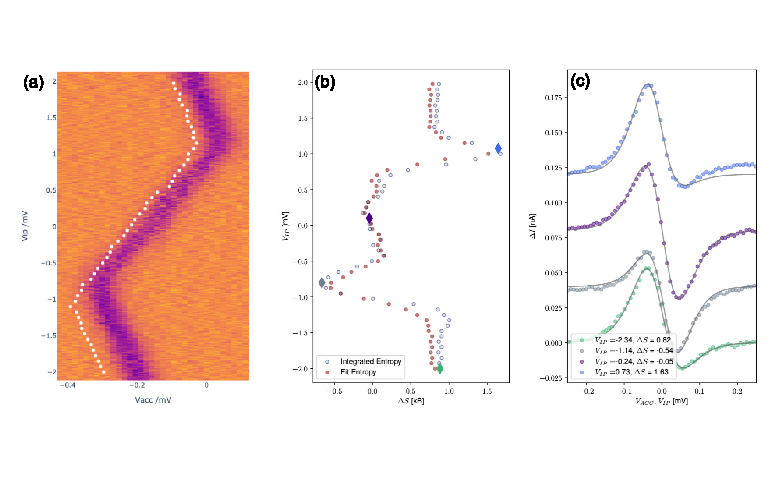
\includegraphics{figures/pdfs/temp_results.eps}}
\caption{Entropy along the 0,1 $\to$ 1,0 transition in the pair of dots. In (a) the dark region indicates the transition in the main quantum dot. White dots indicate the locations where entropy scans were taken. In (b) the $\Delta S$ of the transition at each white point is plotted. In the 0,0 $\to$ 1,0 regime, the $\Delta S$ is found to be roughly $\ln 2 = 0.69$ as expected from the spin degeneracy in the probe dot. In the central regime, where there is a full 0,1 $\to$ 1,0 transition, entropy is found to be around $\ln 2 - \ln2 = 0$ since the spin degeneracy of the impurity dot is simply replaced by the spin degeneracy in the probe dot. In the mixed regime, charge degeneracies of the transitions yield non-trivial $\Delta S$. In (c) the dN/dT signals that were used to calculate these changes in entropy are shown, along with fits.}

\label{fig:results1}       % Give a unique label to the figure. 
\end{figure}

\begin{figure}[h]
\centering
\resizebox{1\textwidth}{!}{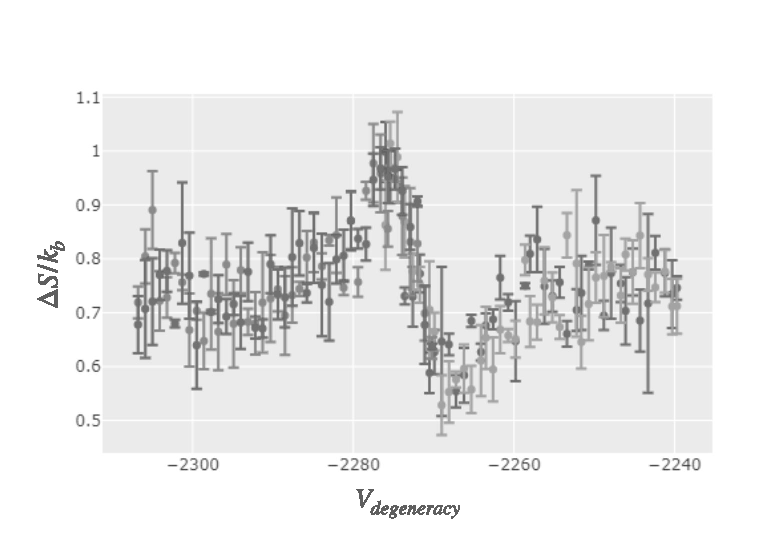
\includegraphics{figures/pdfs/temp_s_shape_bw.eps}}
\caption{ Data from an older device exhibits a change in entropy as degeneracy of an unknown external impurity is adjusted. The demonstrates the potential for measuring the entropy of capacitively coupled systems.}

\label{fig:sshape}       % Give a unique label to the figure. 
\end{figure}



\section{Comparison to theory}
\label{sec:discussion}

The focus of this section will be a comparison between Fig. \ref{fig:results1} and Fig. \ref{fig:yigal_theory} and a qualitative explanation for the effects that we see. In addition, a discussion of the techniques used to make the theoretical predictions.

\begin{figure}[h]
\centering
\resizebox{\textwidth}{!}{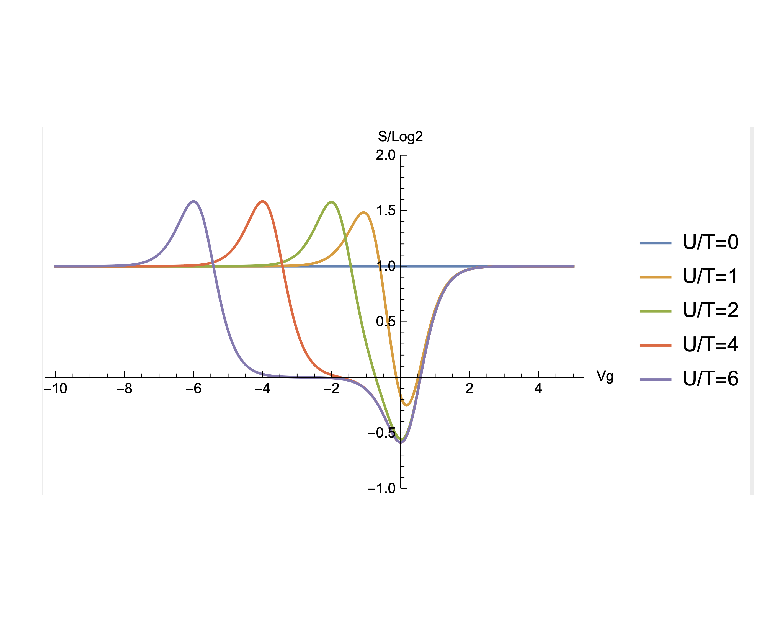
\includegraphics{figures/pdfs/yigal_theory.eps}}
\caption{Theoretical calculations of $\Delta S$ across the 01 $\to$ 10 transition are show for various levels of interdot capacitive coupling to temperature ratios. Excellent alignment with experiment is achieved in the U/T = 6 are achieved.}

\label{fig:yigal_theory}       % Give a unique label to the figure. 
\end{figure}

\section{Conclusion}
\label{sec:conclusion}

Not yet sure what the focus of this section will be, still thinking about it. 


\begin{figure}[h]
\centering
\resizebox{0.5\textwidth}{!}{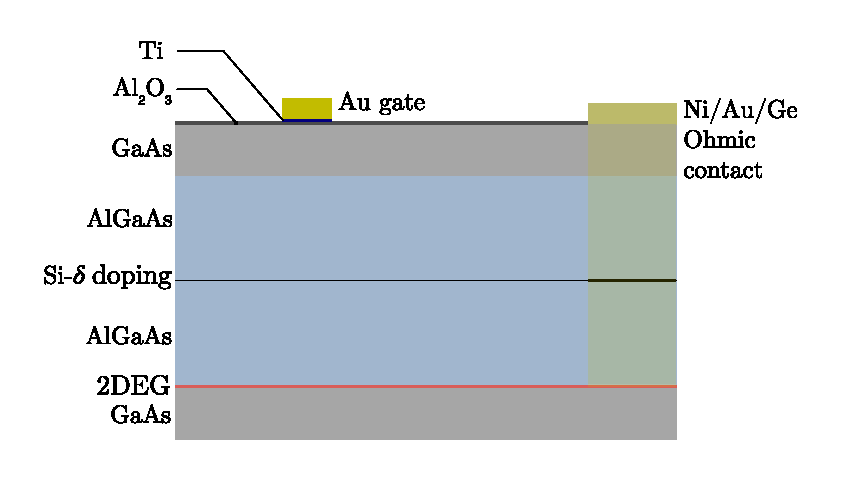
\includegraphics{figures/pdfs/algaas.eps}}
\caption{ A cross section of the GaAs/AlGaAs heterostructure hosting a 2-dimensional electron gas (2DEG) formed at the boundary between an AlGaAs and GaAs layer where the conductance band briefly falls below the Fermi energy \cite{Baer}. Gold gates allow local control of the electron density of the 2DEG. Ohmic contact to the 2DEG is established by a diffusion of a combination of Ni/Au/Ge from the surface to the 2DEG.}

\label{fig:algaas}       % Give a unique label to the figure. 
\end{figure}

\endinput

Any text after an \endinput is ignored.
You could put scraps here or things in progress.
